\documentclass{article}\usepackage[]{graphicx}\usepackage[]{color}
%% maxwidth is the original width if it is less than linewidth
%% otherwise use linewidth (to make sure the graphics do not exceed the margin)
\makeatletter
\def\maxwidth{ %
  \ifdim\Gin@nat@width>\linewidth
    \linewidth
  \else
    \Gin@nat@width
  \fi
}
\makeatother

\definecolor{fgcolor}{rgb}{0.345, 0.345, 0.345}
\newcommand{\hlnum}[1]{\textcolor[rgb]{0.686,0.059,0.569}{#1}}%
\newcommand{\hlstr}[1]{\textcolor[rgb]{0.192,0.494,0.8}{#1}}%
\newcommand{\hlcom}[1]{\textcolor[rgb]{0.678,0.584,0.686}{\textit{#1}}}%
\newcommand{\hlopt}[1]{\textcolor[rgb]{0,0,0}{#1}}%
\newcommand{\hlstd}[1]{\textcolor[rgb]{0.345,0.345,0.345}{#1}}%
\newcommand{\hlkwa}[1]{\textcolor[rgb]{0.161,0.373,0.58}{\textbf{#1}}}%
\newcommand{\hlkwb}[1]{\textcolor[rgb]{0.69,0.353,0.396}{#1}}%
\newcommand{\hlkwc}[1]{\textcolor[rgb]{0.333,0.667,0.333}{#1}}%
\newcommand{\hlkwd}[1]{\textcolor[rgb]{0.737,0.353,0.396}{\textbf{#1}}}%
\let\hlipl\hlkwb

\usepackage{framed}
\makeatletter
\newenvironment{kframe}{%
 \def\at@end@of@kframe{}%
 \ifinner\ifhmode%
  \def\at@end@of@kframe{\end{minipage}}%
  \begin{minipage}{\columnwidth}%
 \fi\fi%
 \def\FrameCommand##1{\hskip\@totalleftmargin \hskip-\fboxsep
 \colorbox{shadecolor}{##1}\hskip-\fboxsep
     % There is no \\@totalrightmargin, so:
     \hskip-\linewidth \hskip-\@totalleftmargin \hskip\columnwidth}%
 \MakeFramed {\advance\hsize-\width
   \@totalleftmargin\z@ \linewidth\hsize
   \@setminipage}}%
 {\par\unskip\endMakeFramed%
 \at@end@of@kframe}
\makeatother

\definecolor{shadecolor}{rgb}{.97, .97, .97}
\definecolor{messagecolor}{rgb}{0, 0, 0}
\definecolor{warningcolor}{rgb}{1, 0, 1}
\definecolor{errorcolor}{rgb}{1, 0, 0}
\newenvironment{knitrout}{}{} % an empty environment to be redefined in TeX

\usepackage{alltt}
\usepackage[sc]{mathpazo}
\usepackage[T1]{fontenc}
\usepackage{geometry}
\geometry{verbose,tmargin=2.5cm,bmargin=2.5cm,lmargin=2.5cm,rmargin=2.5cm}
\setcounter{secnumdepth}{2}
\setcounter{tocdepth}{2}
\usepackage{url}
\usepackage[unicode=true,pdfusetitle,
 bookmarks=true,bookmarksnumbered=true,bookmarksopen=true,bookmarksopenlevel=2,
 breaklinks=false,pdfborder={0 0 1},backref=false,colorlinks=false]
 {hyperref}
\hypersetup{pdfstartview={XYZ null null 1}}
\usepackage{breakurl}
\usepackage{graphicx}
\IfFileExists{upquote.sty}{\usepackage{upquote}}{}
\begin{document}


\title{Advertising Data Report}
\author{Lily Li}
\maketitle

\section{Abstract}

This reports attempts to reproduce the results of advertising and sales found in section 3.1 Simple Linear Regression of An Introduction to Statistical Learning: \url{http://www-bcf.usc.edu/~gareth/ISL/ISLR%20Sixth%20Printing.pdf}.


\section{Introduction}

The Advertising dataset contains data on sales (in thousands of units) for a particular product as a function of advertising budgets (in thousands of dollars) for TV, radio, and newspaper media. The goal is to suggest, on the basis of this data, a marketing plan for next year that will results in high product sales. In this report, we will focus specifcally on the TV budget and its relationship with sales. Some questions we would like to explore include:

\begin{itemize}
\item What are the average TV ads budget and average sales in this dataset?
\item Is there a relationship between TV ads budget and sales?
\item How strong is the relationship?
\item Is the relationship linear?  
\end{itemize}


\section{Data}

This dataset has information on TV, Radio, and Newspaper budgets. On this paper, we will focus on the relationship between \emph{TV budget} and \emph{product sales}.  

Some preliminary analysis of the dataset include:  

\begin{itemize}
\item there are 200 observations of each TV budget and sales
\item histograms below show the distribution of TV budget and sales data
\end{itemize}

\begin{figure}
\centering
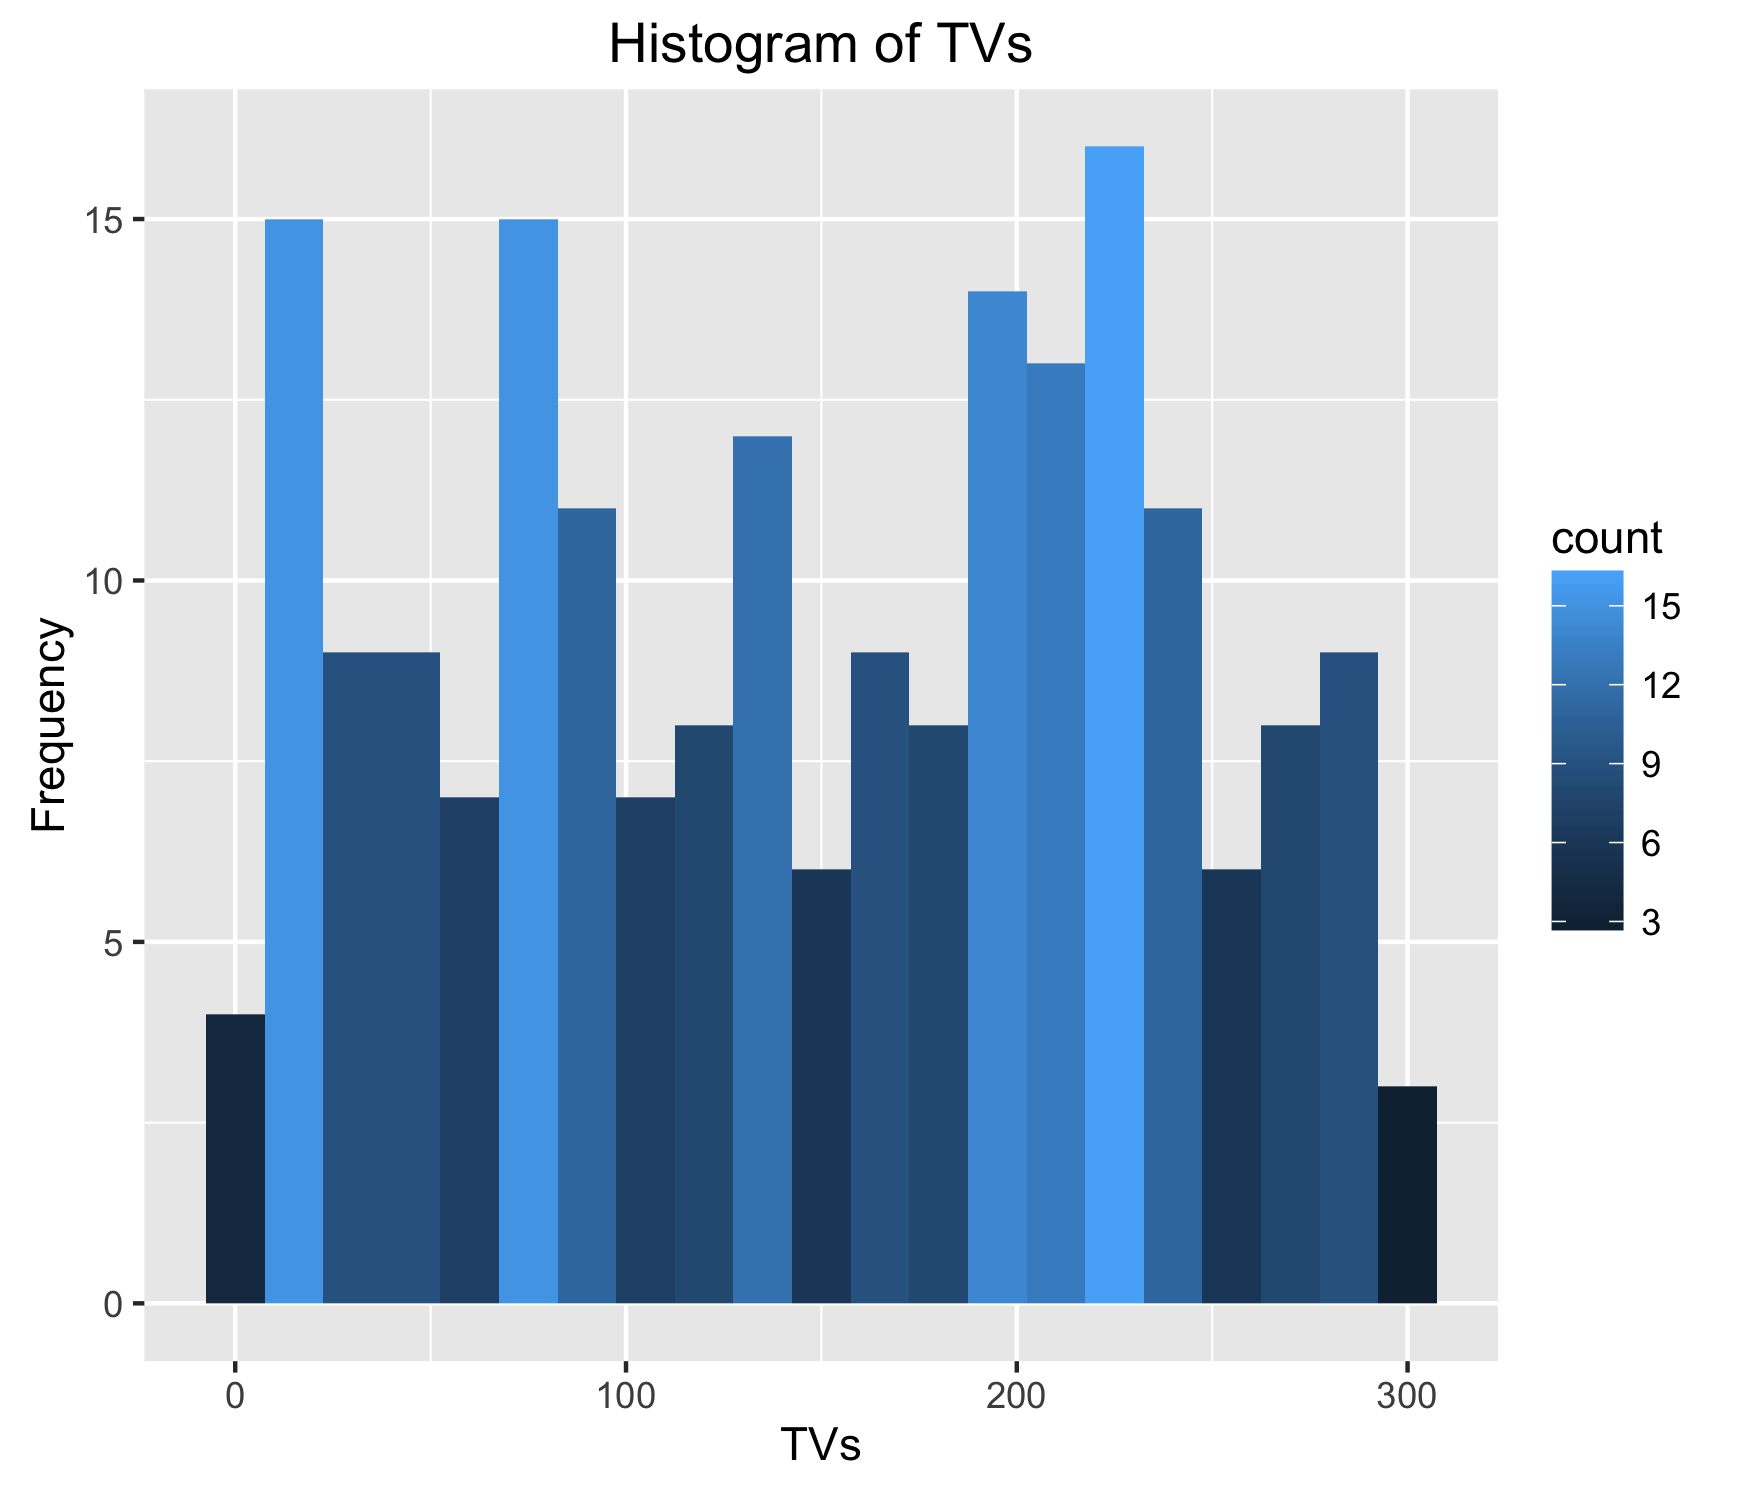
\includegraphics[%
width=0.5\textwidth]{histogram-tv.png}
\caption{\label{fig:DsnTV}Distributions of TV Budget.}
\end{figure}

\begin{figure}
\centering
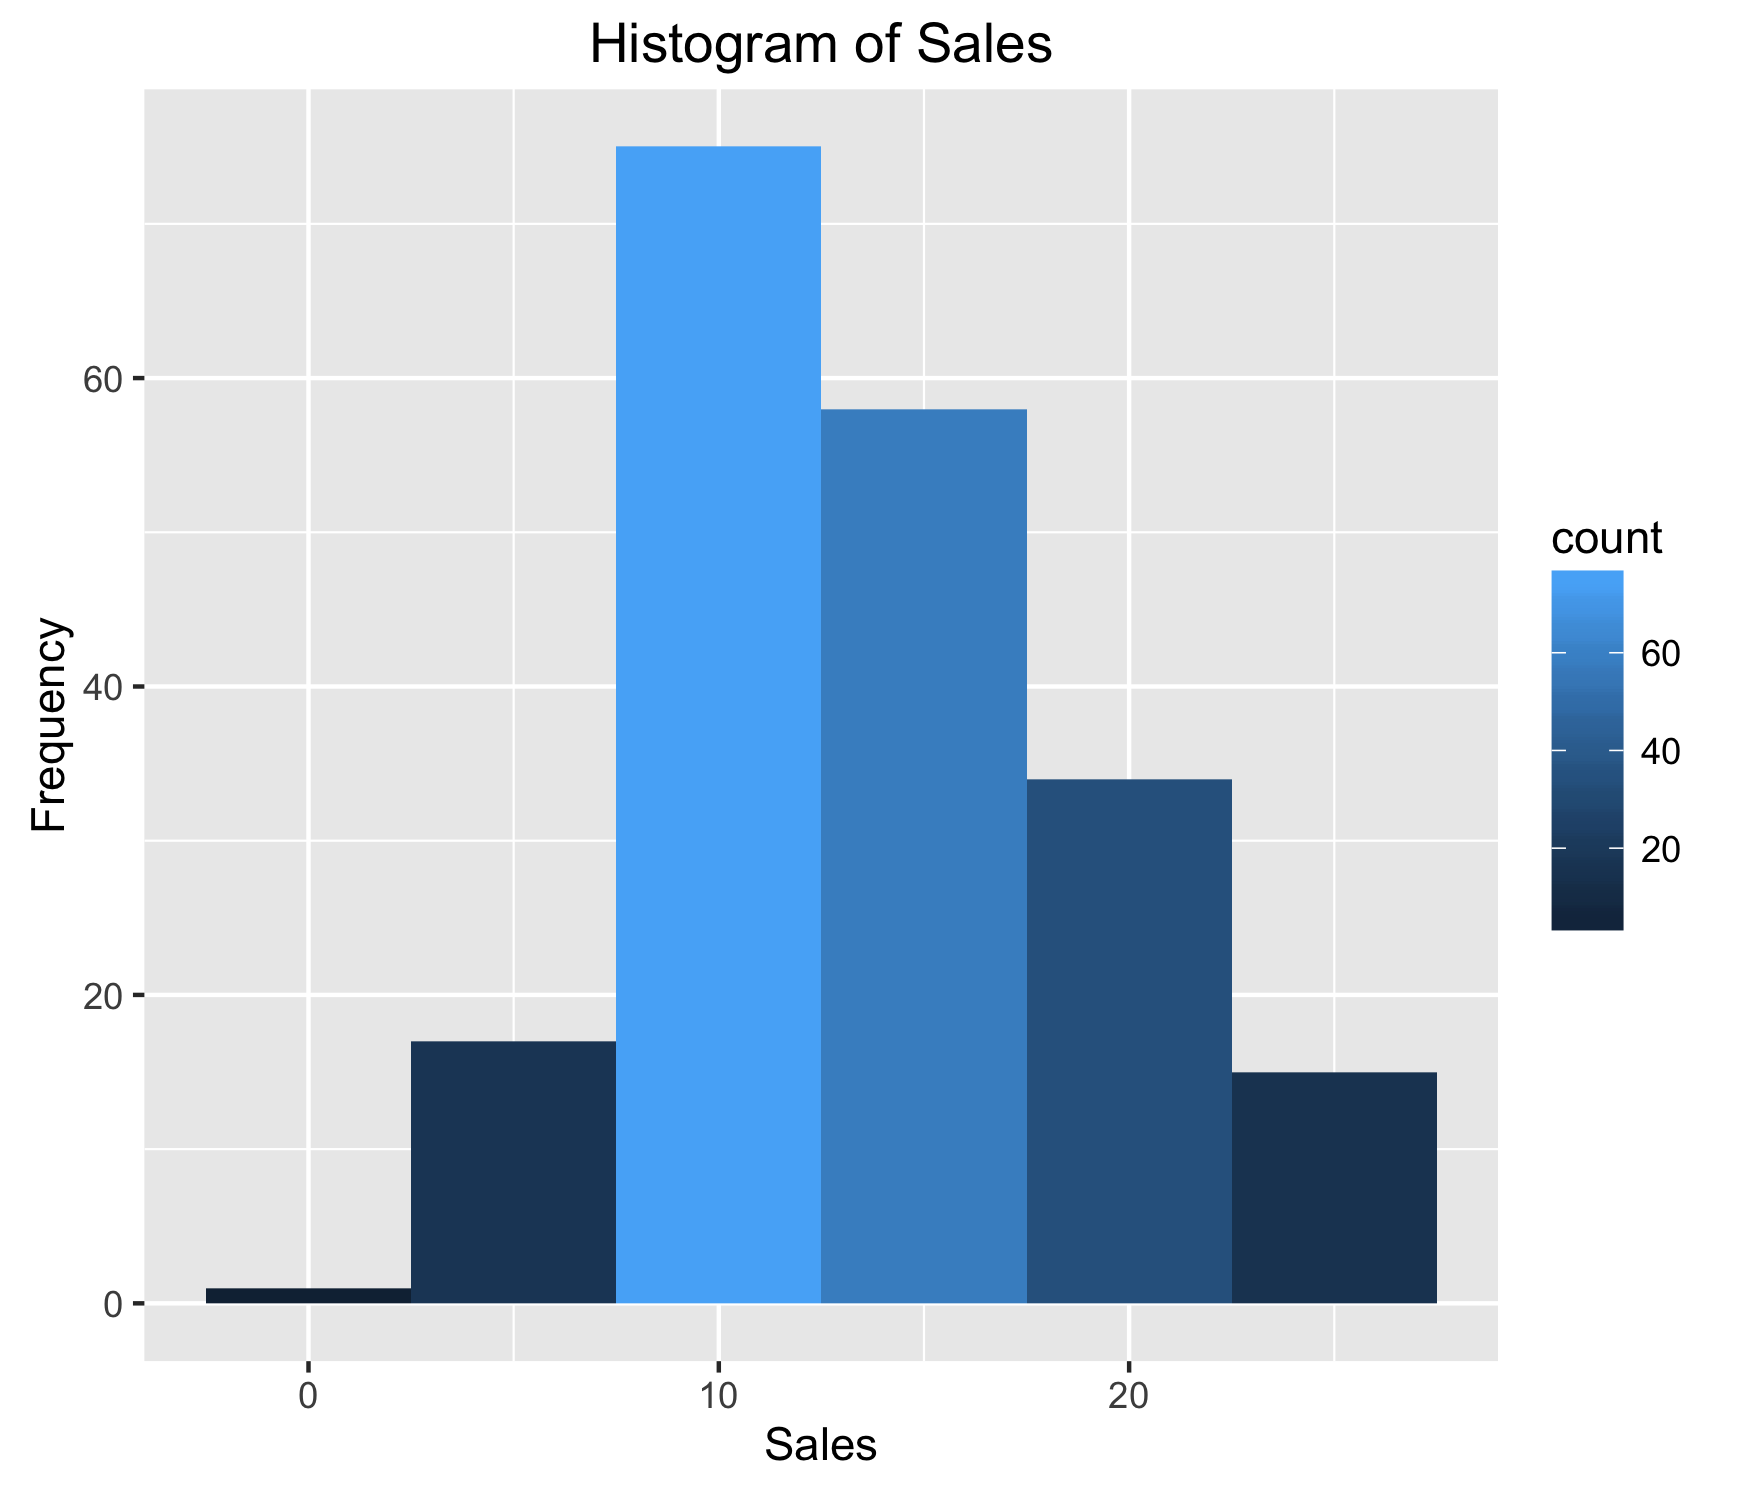
\includegraphics[%
width=0.5\textwidth]{histogram-sales.png}
\caption{\label{fig:DsnSales}Distributions of Sales.}
\end{figure}

\section{Methodology}

We want to observe if there is a linear relationship between TV budget and Sales. Let's consider the regression model: 
\begin{equation}
Sales = \beta_0 + \beta_1 TV
\end{equation}

To estimate the coefficients $\beta_0$ and $\beta_1$, we use the least squares minimization method. 


\section{Results}


After computing the regression, we found the following results: 

% latex table generated in R 3.3.1 by xtable 1.8-2 package
% Mon Oct 31 10:49:56 2016
\begin{table}[ht]
\centering
\begin{tabular}{rrrrr}
  \hline
 & Estimate & Std. Error & t value & Pr($>$$|$t$|$) \\ 
  \hline
(Intercept) & 7.0326 & 0.4578 & 15.36 & 0.0000 \\ 
  TV & 0.0475 & 0.0027 & 17.67 & 0.0000 \\ 
   \hline
\end{tabular}
\end{table}
% latex table generated in R 3.3.1 by xtable 1.8-2 package
% Mon Oct 31 10:49:56 2016
\begin{table}[ht]
\centering
\begin{tabular}{rr}
  \hline
 & Value \\ 
  \hline
r\_squared & 0.61 \\ 
  f\_stat & 312.14 \\ 
  rse & 3.26 \\ 
   \hline
\end{tabular}
\end{table}



\begin{figure}
\centering
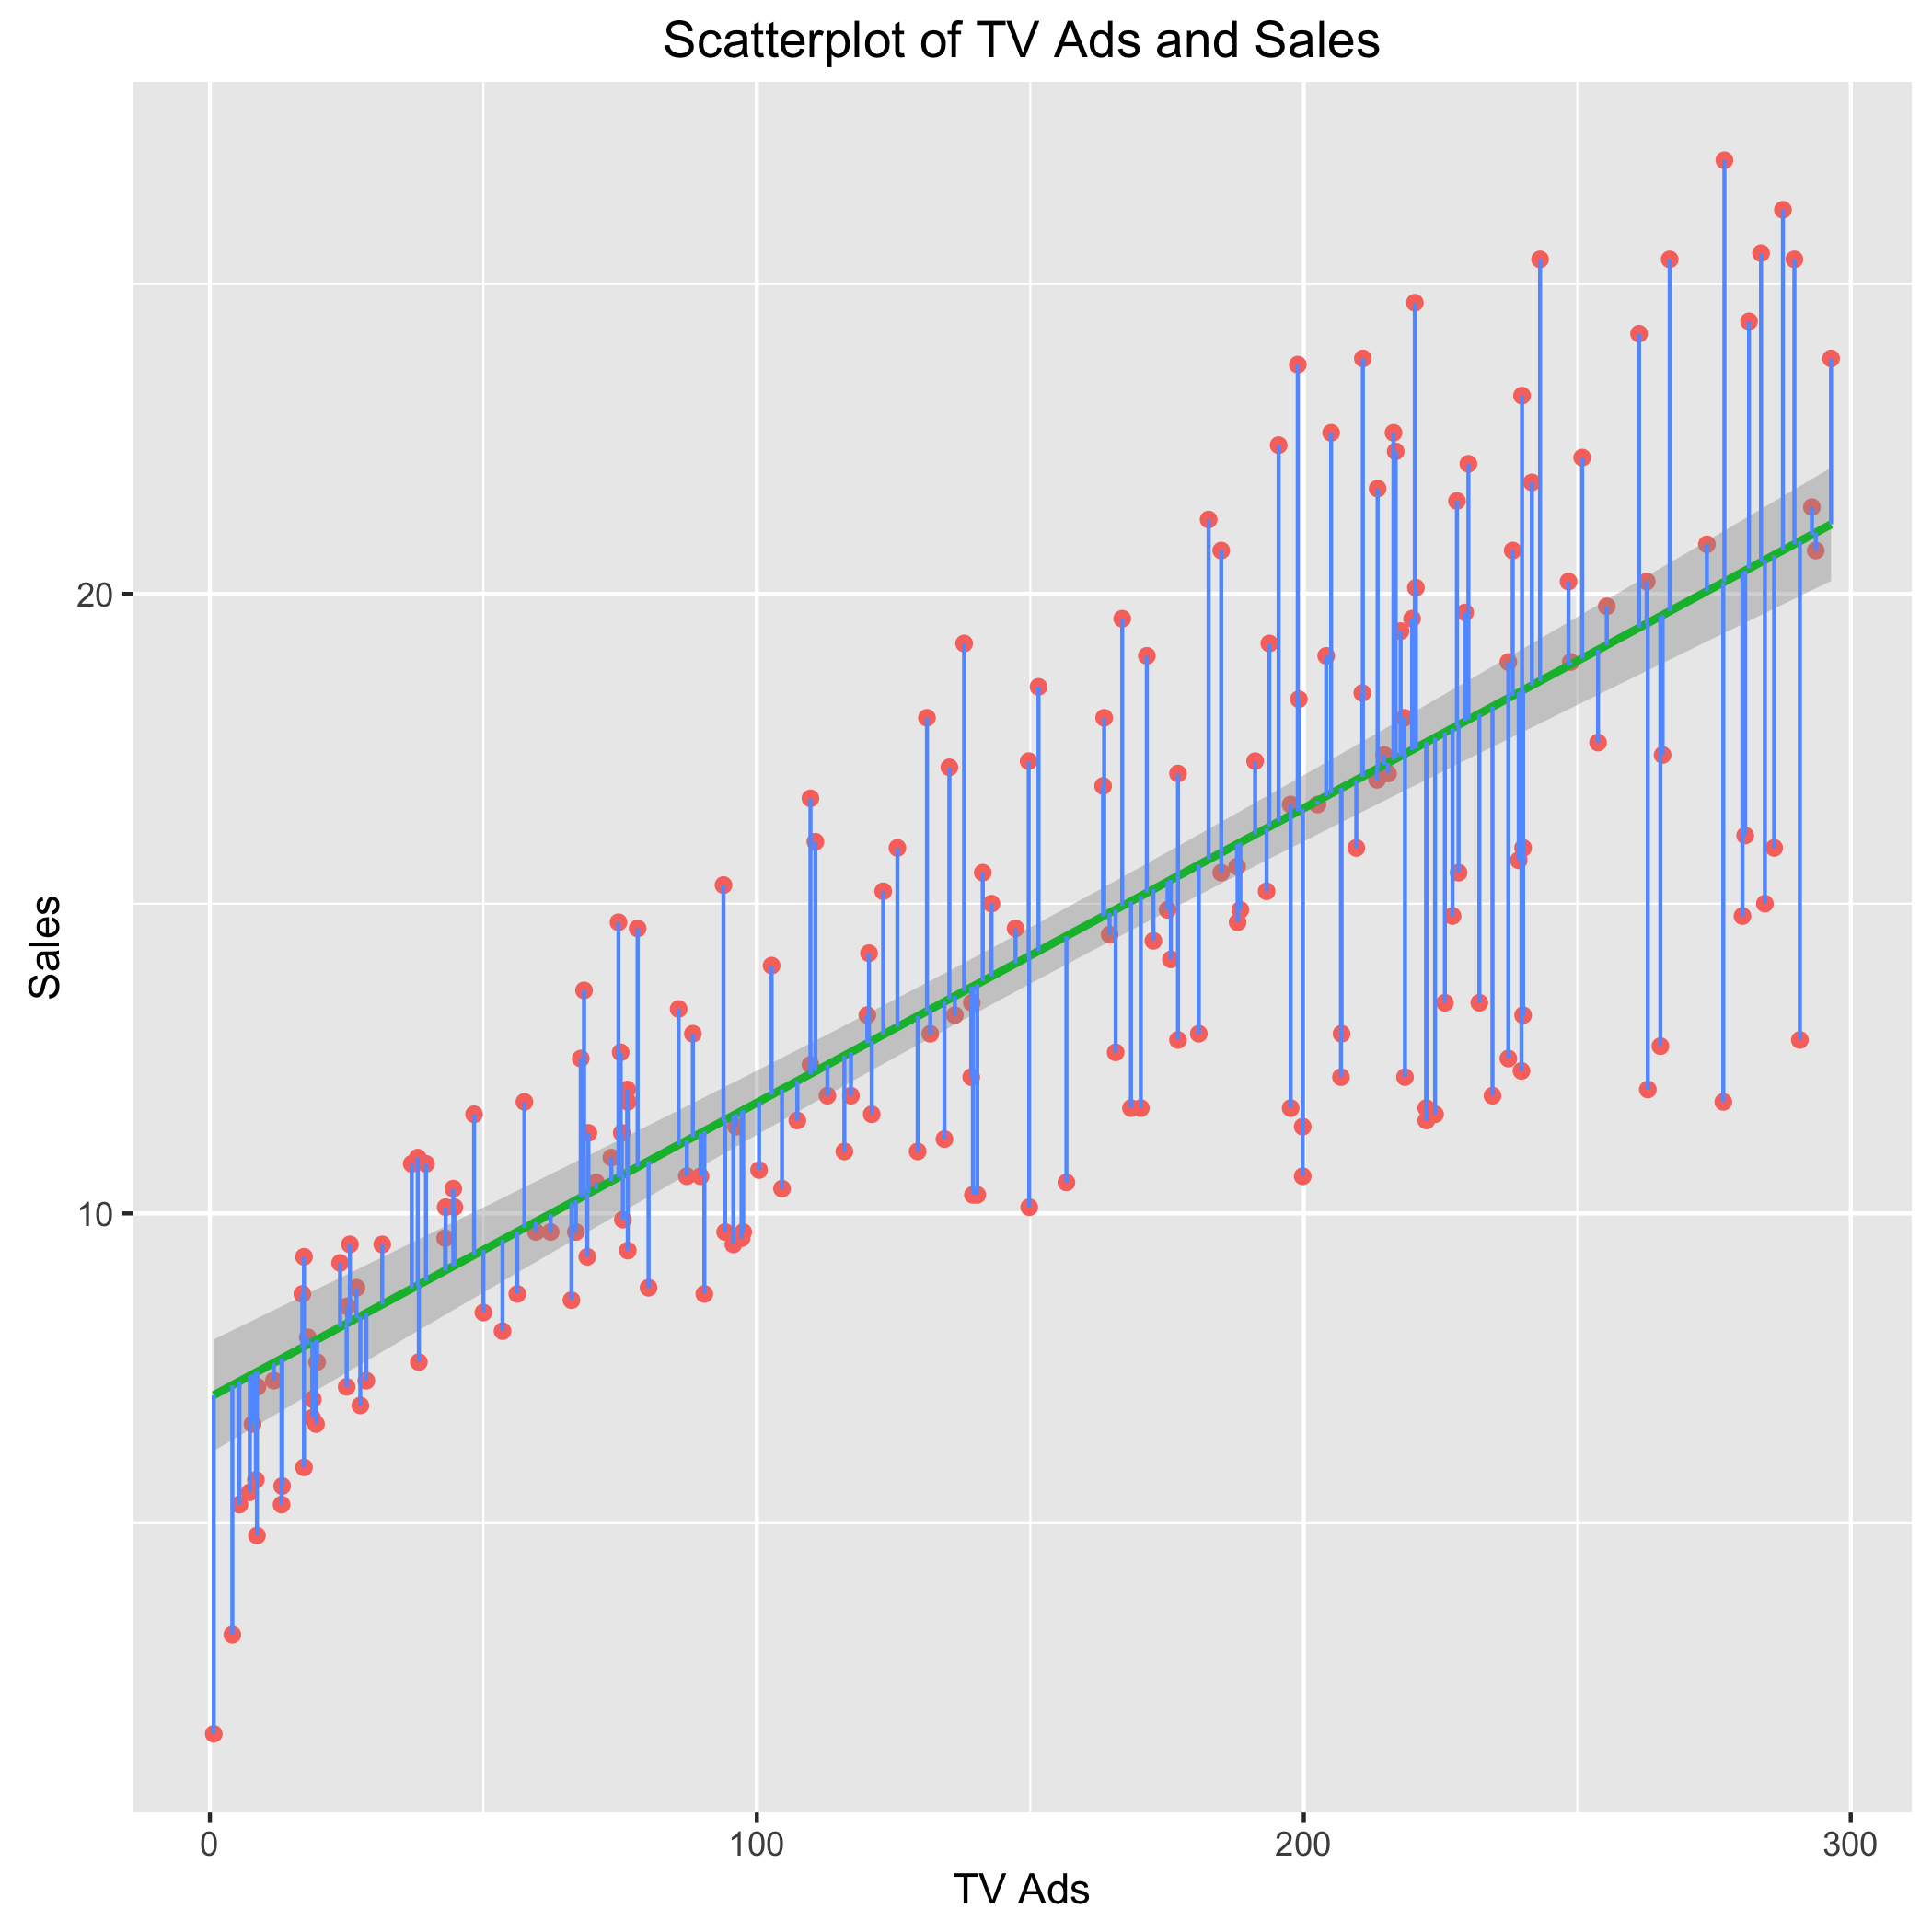
\includegraphics[%
width=0.5\textwidth]{scatterplot-tv-sales.png}
\caption{\label{fig:Scatter}Scatterplot of TV and Sales.}
\end{figure}



\section{Conclusion}

Looking at the TV regression coefficent in Table 1 shows a positive relationship with sales. In fact, 1 percent increase in TV budget is associated with 4.75 percent increase in sales. The t statistic of this coefficient is so large that the p-value is less than 4 decimal places of 0. This coefficient is statistically significant.  

The R squared in Table 2 shows that 61 percent of the variation in sales is explained by the variation in TV budget.   

However, looking at the scatterplot (Figure 2), sales seems to vary more with a higher TV budget and when budget is near 0, sales seem to grow expoentially with TV budget. The data is not homoscedastic and other types of regression might be worth exploring.   


\end{document}
